\documentclass[a4paper,10pt]{article}
\usepackage[utf8]{inputenc}
\usepackage[margin=1.5cm, bottom=2cm]{geometry}
\usepackage{fancyhdr}
\usepackage{enumitem}
\usepackage{amsmath}
\usepackage{amssymb}
\usepackage{xcolor}
\usepackage{makeidx}
\usepackage[most]{tcolorbox}
\newtcolorbox{osservazioni}{
  colback=gray!8,    % sfondo grigio chiaro
  colframe=white,      % nessun bordo
  arc=2mm,            % angoli smussati
  boxrule=0pt,        % spessore bordo 0
  fontupper=\footnotesize,
  left=2mm, right=2mm, top=2mm, bottom=2mm,
  before skip=7pt,   % niente spazio prima
  after skip=15pt     % niente spazio dopo
}
\newtcolorbox{osservazioni2}{
  colback=gray!8,    % sfondo grigio chiaro
  colframe=white,      % nessun bordo
  arc=2mm,            % angoli smussati
  boxrule=0pt,        % spessore bordo 0
  fontupper=\small,
  left=5mm, right=5mm, top=3mm, bottom=3mm,
  before skip=0pt,   % niente spazio prima
  after skip=30pt     % niente spazio dopo
}
\pagestyle{fancy}
\usepackage{tikz}
\usetikzlibrary{automata, positioning}
\pagestyle{fancy}

\usepackage{makeidx}

%%%%%%%%%%%%%%%%%%%
\newcommand{\EsercitazioneNum}{02}
\newcommand{\Data}{02/10/2025}
\newcommand{\DocType}{Esercitazione} % o "Eserciziario"
\newcommand{\FullTitle}{\DocType\ \EsercitazioneNum}

\newcommand{\Header}{
\noindent
  \small \textbf{Computabilità, Complessità e Logica - a.a. 2025/26} \hfill \textbf{\FullTitle} \\[0.2cm]
  \scriptsize Matteo Liotta, \texttt{matteo.liotta@studenti.units.it} \hfill \Data \\[0.2cm]
  \noindent\makebox[\linewidth]{\rule{\linewidth}{0.4pt}} \\[0.3cm]}

\newcommand{\NewPageHeader}{
  \vfill
  \noindent\makebox[\linewidth]{\rule{\linewidth}{0.4pt}}
  \newpage
  {\Header}
}
%%%%%%%%%%%%%%%%%%%

% Numero di pagina in basso al centro
\fancyhf{}
\fancyfoot[C] \thepage
\renewcommand{\footrulewidth}{0pt} % niente linea in basso
\renewcommand{\headrulewidth}{0pt} % niente linea in alto

\begin{document}

\footnotesize  % font generale più piccolo
\Header\\[0.7cm]


%%%%%%%%%%%%%%%% FOGLIO 2


%% INDEX
\addcontentsline{toc}{section}{Esercitazione 02: \textit{Macchine a stati finiti e Linguaggi Regolari (cont'd)}} 
%%
\noindent\Large \textbf{Esercitazione \EsercitazioneNum}: \textit{Macchine a stati finiti e Linguaggi Regolari (cont'd)}\\[0cm]
%\\[0.4cm]
\begin{osservazioni2}
    \textbf{Pumping Lemma}\\
    Dato $L$ linguaggio regolare definito su $\Sigma$, $\exists p \in \mathbb{N}$ (i.e. \emph{pumping length}) tale che, per ogni $w \in L$ con $|w|\geq p$, si ammette la scrittura:
    $$w = xyz$$
    con:
    \begin{itemize}
        \item $|xy| \leq p$,
        \item $|y| > 0$,
    \end{itemize}
    per cui $$\forall i \geq 0,\; x y^i z \in L$$
\end{osservazioni2}


{\normalsize
\begin{itemize}[label=, leftmargin=0pt]

    %% INDEX
    \addcontentsline{toc}{subsection}{Esercizio 8.} 
    %%
    \item \textbf{Esercizio 8 (*)}\\ Sia $L$ linguaggio regolare su $\Sigma=\{a,b\}$, tale per cui 
    {\begin{center}
        $L = \{ w \in \Sigma^* \mid w = a^nb^m,\ \ \  n,m\geq0 \}$
    \end{center}} 
    Dimostrare la regolarità o la non regolarità di tale linguaggio.\\[0.1cm]

    \begin{osservazioni}
        \underline{\textit{Soluzione.}}\\
        Osservando l'indipendenza in numero delle due quantità $a$ e $b$, il linguaggio è atteso quale regolare. Possiamo mostrare tale caratterizzazione disegnando l'automa in grado di riconoscerlo.
            {
    \small
    \begin{center}
    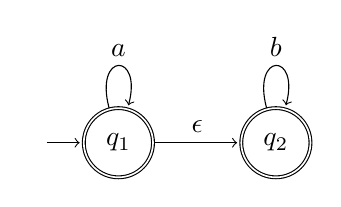
\begin{tikzpicture}[shorten >=1pt, node distance=2cm, on grid, auto]
        \node[state, initial, initial text=,accepting] (q1)   {$q_1$};
        \node[state, accepting] (q2) [right=of q1] {$q_2$};
        
        \path[->]
        (q1) edge [loop above] node {$a$} (q1)
             edge node {$\epsilon$} (q2)
        (q2) edge [loop above] node {$b$} (q2);
        
         
    \end{tikzpicture}
    \end{center}
    }
    \end{osservazioni}

    %% INDEX
    \addcontentsline{toc}{subsection}{Esercizio 9.} 
    %%
    \item \textbf{Esercizio 9. (*)}\\ Sia $L$ linguaggio su $\Sigma=\{a,b\}$, tale per cui 
    {\begin{center}
        $L = \{ w \in \Sigma^* \mid w = a^kb^n, k<n, \ \ \ n\geq 0\}$
    \end{center}} 
    Dimostrare la regolarità o la non regolarità di tale linguaggio.\\[0.1cm]

    \begin{osservazioni}
        \underline{\textit{Soluzione.}}\\
        Poiché si ha la necessità di \textit{ricordare} il numero di $a$ e $b$ che sono state inserite, ci aspettiamo la non regolarità del linguaggio. Se regolare, allora $\exists p\in \mathbf{N}$ tale per cui L dovrebbe ammettere, per ogni sua parola maggiore di $p$ \textbf{pumping length}$$w\in \Sigma^* \quad t.c.\quad |w|>p$$ per ogni scomposizione $$w=x\cdot y \cdot z$$ che soddisfi le condizioni di cui sopra, anche $$w_i=x\cdot y^i \cdot z \in L$$
        Eppure, scegliendo la parola $$w=a^{p}b^{p+1}\in L$$si nota che per ogni scomposizione della forma $$x\cdot y \cdot z$$ 
    \end{osservazioni}

        
    \vfill
    \noindent\makebox[\linewidth]{\rule{\linewidth}{0.4pt}}
    \newpage
    {\noindent
    \small \textbf{Computabilità, Complessità e Logica - a.a. 2025/26} \hfill \textbf{Esercitazione \EsercitazioneNum} \\[0.2cm]
    \scriptsize Matteo Liotta, \texttt{matteo.liotta@studenti.units.it} \hfill \Data \\[0.2cm]
    \noindent\makebox[\linewidth]{\rule{\linewidth}{0.4pt}} \\[0.3cm]}


    \begin{osservazioni}
        comporta che $x\cdot y$ sia \textbf{interamente costituito di simboli $a$}. Dunque anche $y$ è costituito interamente di $a$.\\\\
        Per tale parola $w$, allora, possiamo mostrare che il corrispondente $w_i$, per $i>1$, \textbf{non appartiene} al linguaggio $L$ (dal momento che con già con $i=2$ il numero di $a$ passa a $p$, con conseguente uguaglianza nel numero di $b$). Il linguaggio non è regolare. 
    \end{osservazioni}

    %% INDEX
    \addcontentsline{toc}{subsection}{Esercizio 10.} 
    %%
    \item \textbf{Esercizio 10. (**)}\\ Si consideri il linguaggio dell'esercizio 5. \textit{(Esercitazione 01)}. Si provi a confermare analiticamente l'intuizione di non regolarità relativa a tale linguaggio. \\[0.1cm]

    \begin{osservazioni}
        \underline{\textit{Soluzione.}}\\
        Il linguaggio in questione è il seguente:
        $$   L = \{ w \in \Sigma^* \mid \#a = \#b\ in\ w\}$$

        Poiché persiste la necessità di \textit{ricordare} il numero di $a$ e $b$ che sono state inserite, ci aspettiamo la non regolarità del linguaggio. Se regolare, allora $\exists p\in \mathbf{N}$ tale per cui L dovrebbe ammettere, per ogni sua parola maggiore di $p$ \textbf{pumping length}$$w\in \Sigma^* \quad t.c.\quad |w|>p$$ per ogni scomposizione $$w=x\cdot y \cdot z$$ che soddisfi le condizioni di cui sopra, anche $$w_i=x\cdot y^i \cdot z \in L$$
        Eppure, scegliendo la parola $$w=a^{p}b^{p}\in L$$si nota che per ogni scomposizione della forma $$x\cdot y \cdot z$$ comporta che $x\cdot y$ sia \textbf{interamente costituito di simboli $a$}. Dunque anche $y$ è costituito interamente di $a$.\\\\
        Per tale parola $w$, allora, possiamo mostrare che il corrispondente $w_i$, per $i>1$, \textbf{non appartiene} al linguaggio $L$ (dal momento che con $i=2$ il numero di $a$ passa a $p+1$, mentre il numero di $b$ resta invariato). Il linguaggio non è regolare. 
        
    \end{osservazioni}

    %% INDEX
    \addcontentsline{toc}{subsection}{Esercizio 11.} 
    %%
    \item \textbf{Esercizio 11 (*)}\\ Sia $L$ linguaggio regolare su $\Sigma=\{a,b,0\}$, tale per cui 
    {\begin{center}
        $L = \{ w \in \Sigma^* \mid w = z00, z \in \Sigma^* \}$
    \end{center}} 
    Dimostrare la regolarità o la non regolarità di tale linguaggio.\\[0.1cm]


    \begin{osservazioni}
        \underline{\textit{Soluzione.}}\\
        Osservando l'indipendenza in numero delle due quantità $a$ e $b$, il linguaggio è atteso quale regolare. Possiamo mostrare tale caratterizzazione disegnando l'automa in grado di riconoscerlo.
            {
    \small
    \begin{center}
    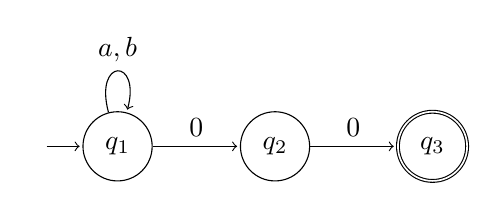
\begin{tikzpicture}[shorten >=1pt, node distance=2cm, on grid, auto]
        \node[state, initial, initial text=] (q1)   {$q_1$};
        \node[state] (q2) [right=of q1] {$q_2$};
        \node[state, accepting] (q3) [right=of q2] {$q_3$};
        
        \path[->]
        (q1) edge [loop above] node {$a,b$} (q1)
             edge node {$0$} (q2)
        (q2) edge node {$0$} (q3);
        
         
    \end{tikzpicture}
    \end{center}
    }
    \end{osservazioni}

     %% INDEX
    \addcontentsline{toc}{subsection}{Esercizio 12.} 
    %%
    \item \textbf{Esercizio 12. (***)}\\ Sia $L$ linguaggio su $\Sigma=\{a,b\}$, tale per cui 
    {\begin{center}
        $L = \{ w \in \Sigma^* \mid w = a^{2^n}, n\geq 0\}$
    \end{center}} 
    Dimostrare la regolarità o la non regolarità di tale linguaggio.\\[0.1cm]

    \vfill
    \noindent\makebox[\linewidth]{\rule{\linewidth}{0.4pt}}
    \newpage
    {\noindent
    \small \textbf{Computabilità, Complessità e Logica - a.a. 2025/26} \hfill \textbf{Esercitazione \EsercitazioneNum} \\[0.2cm]
    \scriptsize Matteo Liotta, \texttt{matteo.liotta@studenti.units.it} \hfill \Data \\[0.2cm]
    \noindent\makebox[\linewidth]{\rule{\linewidth}{0.4pt}} \\[0.3cm]}



    \begin{osservazioni}
        \underline{\textit{Soluzione.}}\\
        Il linguaggio in questione è costituito delle seguenti parole:
        \begin{itemize}
            \item $a^{2^0}\quad =\quad a$
            \item $a^{2^1}\quad =\quad aa$
            \item $a^{2^2}\quad =\quad aaaa$
            \item $a^{2^3}\quad =\quad aaaaaaaa$
            \item $a^{2^4}\quad =\quad aaaaaaaaaaaaaaaa$
            \item $a^{2^5}\quad =\quad aaaaaaaaaaaaaaaaaaaaaaaaaaaaaaaa$
            \item $...$
            
        \end{itemize}

        Ci aspettiamo la non regolarità del linguaggio. Se regolare, allora $\exists p\in \mathbf{N}$ tale per cui L dovrebbe ammettere, per ogni sua parola maggiore di $p$ \textbf{pumping length}$$w\in \Sigma^* \quad t.c.\quad |w|>p$$ per ogni scomposizione $$w=x\cdot y \cdot z$$ che soddisfi le condizioni di cui sopra, anche $$w_i=x\cdot y^i \cdot z \in L$$
        
        Scegliamo di considerare la parola $$w=a^{2^p}\in L$$
        
        Supponiamo che $w$ sia scomposto, \textbf{senza perdere di generalità}, nella seguente maniera:
        $$w=a^{2^p} = a^k\cdot a^t \cdot a^{2^p-k-t}$$
        con 
        \begin{itemize}
            \item $x=a^k$
            \item $y = a^t$
            \item $k+t\leq p$
        \end{itemize}
        Si noti ancora una volta che non abbiamo fissato nessun caso specifico, ma solamente esplicitato formalmente che $x$ ed $y$ saranno costituite da un numero arbitrario di $a$.
        A questo punto, il pumping lemma ammette che 
        $\forall i\geq 0, \quad w_i=x\cdot y^i \cdot z \in L$
        con 
        $$w_i=x\cdot y^i \cdot z=a^k \cdot (a^t)^i \cdot a^{2^p -k-t}, \quad k+t\leq p$$
        Se così allora:
        $$w_i=a^{k+it+2^p-k-t}=a^{2^p+(i-1)t}$$
        Si osservi come però
        $$k+t\leq p \Leftrightarrow t\leq p-k< p,\quad t>0$$
        Ed è noto come
        $$a^{2^{p+1}} = a^{2^{p}} \cdot a^{2^{p}}> a^{2^p}a^{p} \quad \forall p\geq1$$
        A questo punto
                $${2^p+(i-1)t} < 2^p+(i-1)p$$
        Che con $i=2$ $${2^p+(i-1)t} < 2^p+(i-1)p = 2^p+p$$
        Quindi, senza formalismi, la parola non è sufficientemente lunga con un $i=2$ (che obbligatoriamente ne deve accrescere la lunghezza) da raggiungere il caso successivo coperto dalla definizione del linguaggio: $a^{2^{p+1}}$. Poichè non avendo perso di generalità esso vale per ogni scomposizione, il linguaggio non può essere regolare.
        

    \end{osservazioni}
    
    

    %% INDEX
    \addcontentsline{toc}{subsection}{Esercizio 13.} 
    %%
    \item \textbf{Esercizio 13. (***)}\\ Sia $L$ linguaggio su $\Sigma=\{a,b\}$, tale per cui 
    {\begin{center}
        $L = \{ w\#w' | w,w'\in \Sigma^* \land w \neq w'\}$
    \end{center}} 
    Dimostrare la regolarità o la non regolarità di tale linguaggio.


    \vfill
    \noindent\makebox[\linewidth]{\rule{\linewidth}{0.4pt}}
    \newpage
    {\noindent
    \small \textbf{Computabilità, Complessità e Logica - a.a. 2025/26} \hfill \textbf{Esercitazione \EsercitazioneNum} \\[0.2cm]
    \scriptsize Matteo Liotta, \texttt{matteo.liotta@studenti.units.it} \hfill \Data \\[0.2cm]
    \noindent\makebox[\linewidth]{\rule{\linewidth}{0.4pt}} \\[0.3cm]}


    \begin{osservazioni}
        \underline{\textit{Soluzione.}}\\

        Si noti che nel linguaggio non è indicato il modo in cui tale differenza tra le parole può essere espressa. Se regolare, allora $\exists p\in \mathbf{N}$ tale per cui L dovrebbe ammettere, per ogni sua parola maggiore di $p$ \textbf{pumping length}$$w\in \Sigma^* \quad t.c.\quad |w|>p$$ per ogni scomposizione $$w=x\cdot y \cdot z$$ che soddisfi le condizioni di cui sopra, anche $$w_i=x\cdot y^i \cdot z \in L$$
        Eppure, scegliendo la parola $$w=a^{p}\#a^{p+1}\in L$$si nota che per ogni scomposizione della forma $$x\cdot y \cdot z$$ comporta che $x\cdot y$ sia \textbf{interamente costituito di simboli $a$}. Dunque anche $y$ è costituito interamente di $a$.\\\\
        Per tale parola $w$, allora, possiamo mostrare che il corrispondente $w_i$, per $i>1$, \textbf{non appartiene} al linguaggio $L$ (dal momento che con $i=2$ il numero di $a$ passa a $p+1$, con conseguente uguaglianza di $w_1$ e $w_2$). Il linguaggio non è regolare. 
        
    \end{osservazioni}

    $$\\$$
    
    \item \textit{\textbf{Esercizi Aggiuntivi}}

    %% INDEX
    \addcontentsline{toc}{subsection}{Esercizio 14.} 
    %%
    \item \textbf{Esercizio 14. (**)}\\ Sia $L$ linguaggio su $\Sigma=\{a,b,c\}$, tale per cui 
    {\begin{center}
        $L = \{ w\in \Sigma^* | w=a^nb^mc^k, \ k>n+m, \ \ n\geq 0, m\geq 0\}$
    \end{center}} 
    Dimostrare la regolarità o la non regolarità di tale linguaggio.\\[0.1cm]

    %% INDEX
    \addcontentsline{toc}{subsection}{Esercizio 15.} 
    %%
    \item \textbf{Esercizio 15. (***)}\\ Sia $L_n$ linguaggio regolare su $\Sigma=\{a,b\}$, tale per cui 
    {\\ \begin{center}
        $L_n = \{ w \in \Sigma^* \mid w = a^k, k\ \%\ n=0\}$
    \end{center}} 
    Si dimostri per $n\geq 1$ è un linguaggio regolare.\\[0.1cm]

    %% INDEX
    \addcontentsline{toc}{subsection}{Esercizio 16.} 
    %%
    \item \textbf{Esercizio 16. (*)}\\
    Si consideri il seguente automa regolare su $\Sigma = \{0,1\}$:
    {
    \small
    \begin{center}
    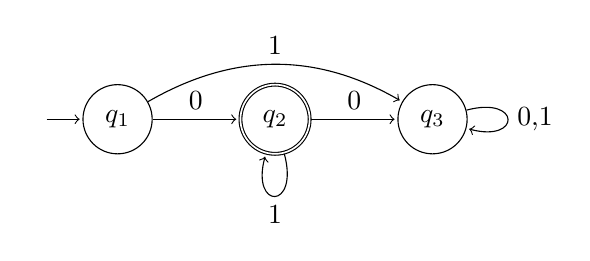
\begin{tikzpicture}[shorten >=1pt, node distance=2cm, on grid, auto]
        \node[state, initial, initial text=] (q1)   {$q_1$};
        \node[state, accepting] (q2) [right=of q1] {$q_2$};
        \node[state] (q3) [right=of q2] {$q_3$};
        
        \path[->]
        (q1) edge [bend left] node {1} (q3)
             edge node {0} (q2)
        (q2) edge [loop below] node {1} ()
             edge node {0} (q3)
        (q3) edge [loop right] node {0,1} ();
         
    \end{tikzpicture}
    \end{center}
    }
    Si identifichi il linguaggio riconosciuto dall'automa.\\[0.1cm]


%\item \textbf{Esercizio 11. (*)}\\
%Si consideri il seguente automa regolare su $\Sigma = \{0,1\}$:
%{
%\small
%\begin{center}
%\begin{tikzpicture}[shorten >=1pt, node distance=2cm, on grid, auto]
%    \node[state, initial, initial text=] (p1)   {$p_1$};
%    \node[state, accepting] (p2) [right=of p1] {$p_2$};
%    \node[state] (p3) [right=of p2] {$p_3$};
%    
%    \path[->]
%    (p1) edge [loop above] node {1} (p1)
%         edge [bend left] node {0} (p2)
%    (p2) edge [loop above] node {0} (p2)
%         edge [bend left] node {1} (p1)
%         edge [bend left] node {1} (p3)
%    (p3) edge [loop above] node {1} (p3)
%         edge [bend left] node {0} (p2)
%    
%\end{tikzpicture}
%\end{center}
%}
%Si identifichi il linguaggio riconosciuto dall'automa.


    \vfill
    \noindent\makebox[\linewidth]{\rule{\linewidth}{0.4pt}}
    \newpage
    {\noindent
    \small \textbf{Computabilità, Complessità e Logica - a.a. 2025/26} \hfill \textbf{Esercitazione \EsercitazioneNum} \\[0.2cm]
    \scriptsize Matteo Liotta, \texttt{matteo.liotta@studenti.units.it} \hfill \Data \\[0.2cm]
    \noindent\makebox[\linewidth]{\rule{\linewidth}{0.4pt}} \\[0.3cm]}

    %% INDEX
    \addcontentsline{toc}{subsection}{Esercizio 17.} 
    %%
    \item \textbf{Esercizio 17. (**)}\\
    Si consideri il seguente automa regolare su $\Sigma = \{a,b,c\}$:
    {
    \small
    \begin{center}
    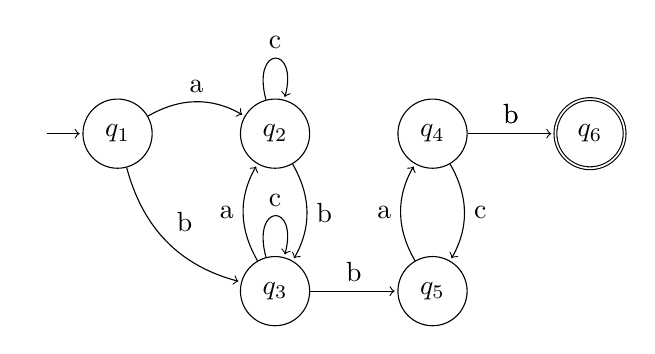
\begin{tikzpicture}[shorten >=1pt, node distance=2cm, on grid, auto]
        
        \node[state] (q2) {$q_2$};
        \node[state, below=of q2] (q3) {$q_3$};

        \node[state, right=of q2] (q4) {$q_4$};
        \node[state, below=of q4] (q5) {$q_5$};
        \node[state, right=of q4, accepting] (q6) {$q_6$};

        \node[state, initial, initial text=, left=of q2] (q1) {$q_1$};

        \path[->]
        (q1) edge [bend left] node {a} (q2)
             edge [bend right] node {b} (q3)
        (q2) edge [bend left] node {b} (q3)
             edge [loop above] node {c} ()
        (q3) edge [bend left] node {a} (q2)
             edge [loop above] node {c} ()
             edge node {b} (q5)
        (q5) edge [bend left] node {a} (q4)
        (q4) edge [bend left] node {c} (q5)
             edge node {b} node {b} (q6);

    \end{tikzpicture}
    \end{center}
    }
    Si identifichi il linguaggio riconosciuto dall'automa.
    
\end{itemize}
}
\vfill
\noindent\makebox[\linewidth]{\rule{\linewidth}{0.1pt}}
\end{document}
